% !TeX program = xelatex
\documentclass[11pt,a4paper]{article}
\usepackage{fontspec}
% File-based Windows font loading avoids MiKTeX's missing-font installer.
\IfFileExists{C:/Windows/Fonts/times.ttf}{%
\setmainfont{times.ttf}[Path=C:/Windows/Fonts/,BoldFont=timesbd.ttf,ItalicFont=timesi.ttf,BoldItalicFont=timesbi.ttf]
\setsansfont{arial.ttf}[Path=C:/Windows/Fonts/,BoldFont=arialbd.ttf,ItalicFont=ariali.ttf,BoldItalicFont=arialbi.ttf]
\setmonofont{consola.ttf}[Path=C:/Windows/Fonts/,BoldFont=consolab.ttf,ItalicFont=consolai.ttf,Scale=MatchLowercase]
}{%
\setmainfont{TeX Gyre Termes}
\setsansfont{TeX Gyre Heros}
\setmonofont{DejaVu Sans Mono}[Scale=MatchLowercase]
}
\usepackage[a4paper,left=25mm,right=23mm,top=24mm,bottom=24mm,headheight=15pt]{geometry}
\usepackage{graphicx,booktabs,tabularx,array,amsmath,float,needspace}
\usepackage[table]{xcolor}
\usepackage{fancyhdr,caption,titlesec,enumitem,tikz,url}
\usetikzlibrary{arrows.meta,positioning}
\definecolor{navy}{HTML}{17324D}
\definecolor{teal}{HTML}{217E87}
\definecolor{pale}{HTML}{EEF3F5}
\definecolor{ink}{HTML}{20262D}
\usepackage[unicode,colorlinks=true,linkcolor=navy,citecolor=teal,urlcolor=teal,bookmarksnumbered=true]{hyperref}
\hypersetup{pdftitle={DocuCheck AI - Báo cáo tiến độ tuần 2},pdfsubject={Báo cáo tiến độ Week 2},pdfauthor={Winner Winner Chicken Dinner: Nguyễn Văn Minh; Nguyễn Thành Trung}}
\renewcommand{\contentsname}{Mục lục}
\renewcommand{\refname}{Tài liệu tham khảo}
\renewcommand{\figurename}{Hình}
\renewcommand{\tablename}{Bảng}
\renewcommand{\thesection}{\Roman{section}}
\renewcommand{\thesubsection}{\arabic{section}.\arabic{subsection}}
\titleformat{\section}{\Large\sffamily\bfseries\color{navy}}{\thesection.}{.6em}{}
\titleformat{\subsection}{\large\bfseries\color{navy}}{\thesubsection}{.6em}{}
\titleformat{\subsubsection}{\normalsize\bfseries\color{navy}}{}{0pt}{}
\titlespacing*{\section}{0pt}{10pt}{12pt}
\titlespacing*{\subsection}{0pt}{13pt}{6pt}
\titlespacing*{\subsubsection}{0pt}{10pt}{4pt}
\setlength{\parindent}{0pt}
\setlength{\parskip}{6pt plus 1pt}
\linespread{1.08}
\setlength{\emergencystretch}{2em}
\raggedbottom
\clubpenalty=10000
\widowpenalty=10000
\AddToHook{cmd/section/before}{\Needspace{5\baselineskip}}
\AddToHook{cmd/subsection/before}{\Needspace{4\baselineskip}}
\setlength{\tabcolsep}{5pt}
\renewcommand{\arraystretch}{1.25}
\newcolumntype{P}[1]{>{\raggedright\arraybackslash}p{#1}}
\newcolumntype{Y}{>{\raggedright\arraybackslash}X}
\captionsetup{font=small,labelfont={bf,color=navy},justification=raggedright,singlelinecheck=false,skip=6pt}
\setlist{nosep,leftmargin=1.3em,topsep=4pt}
\pagestyle{fancy}
\fancyhf{}
\fancyhead[L]{\small\sffamily\color{navy}DOCUCHECK AI}
\fancyhead[R]{\small\sffamily\color{navy}BÁO CÁO TUẦN 2}
\fancyfoot[L]{\footnotesize\color{navy}Báo cáo tiến độ tuần 2 \enspace | \enspace 06.11.2026}
\fancyfoot[R]{\small\thepage}
\renewcommand{\headrulewidth}{.4pt}
\newcommand{\note}[1]{\par\begingroup\setlength{\fboxsep}{9pt}\noindent\colorbox{pale}{\parbox{\dimexpr\linewidth-18pt\relax}{#1}}\endgroup\par}
\urlstyle{tt}
\makeatletter
\g@addto@macro\UrlBreaks{\do\a\do\b\do\c\do\d\do\e\do\f\do\g\do\h\do\i\do\j\do\k\do\l\do\m\do\n\do\o\do\p\do\q\do\r\do\s\do\t\do\u\do\v\do\w\do\x\do\y\do\z\do\A\do\B\do\C\do\D\do\E\do\F\do\G\do\H\do\I\do\J\do\K\do\L\do\M\do\N\do\O\do\P\do\Q\do\R\do\S\do\T\do\U\do\V\do\W\do\X\do\Y\do\Z\do\0\do\1\do\2\do\3\do\4\do\5\do\6\do\7\do\8\do\9}
\makeatother
\begin{document}
\color{ink}

\begin{titlepage}
\thispagestyle{empty}
\centering
\setlength{\parskip}{0pt}
\vspace*{7mm}
{\sffamily\fontsize{16}{21}\selectfont\bfseries\color{navy}AI-VIETNAM}\par
\vspace{3mm}
{\sffamily\fontsize{11}{16}\selectfont KHÓA HỌC AIO2026}\par
\vspace{7mm}
{\color{navy!35}\rule{72mm}{.45pt}}\par
\vspace{25mm}
{\fontsize{23}{31}\selectfont\bfseries\color{navy}BÁO CÁO TIẾN ĐỘ TUẦN 2}\par
\vspace{5mm}
{\sffamily\fontsize{12}{17}\selectfont\color{teal}Đánh giá OCR và phân tích lỗi}\par
\vspace{17mm}
{\fontsize{29}{35}\selectfont\bfseries\color{navy}DocuCheck AI}\par
\vspace{3mm}
{\fontsize{14}{19}\selectfont Hệ thống xử lý và kiểm tra tài liệu}\par
\vspace{7mm}
{\fontsize{11}{16}\selectfont\itshape
Benchmark crop, phân đoạn trang và so sánh ba engine}\par
\vspace{24mm}
\begin{minipage}{114mm}
\normalsize
\renewcommand{\arraystretch}{1.65}
\begin{tabularx}{\linewidth}{@{}P{32mm}Y@{}}
\textbf{Tên nhóm} & Winner Winner Chicken Dinner\\
\textbf{Thành viên 1} & Nguyễn Văn Minh\\
\textbf{Thành viên 2} & Nguyễn Thành Trung\\
\end{tabularx}
\end{minipage}
\vfill
{\small Ngày lập báo cáo: 06 tháng 11 năm 2026}\par
\vspace{6mm}
{\footnotesize\href{https://github.com/AIVIETNAM-AIO-Heart208/DocuCheck-AI}{\textsf{github.com/AIVIETNAM-AIO-Heart208/DocuCheck-AI}}}\par
\vspace*{8mm}
\end{titlepage}

\section*{Tóm tắt}
Trong tuần 2, nhóm chuyển từ khảo sát dữ liệu và thiết lập OCR ban đầu sang đánh giá có kiểm soát. Ba hướng thực hiện gồm: xây dựng benchmark nhận dạng trên ảnh cắt nhỏ (crop), so sánh chế độ phân đoạn trang của Tesseract và đối chiếu ba engine nhận dạng tiếng Việt. Các thí nghiệm trả lời những câu hỏi khác nhau, vì vậy kết quả được trình bày riêng theo tập dữ liệu và quy tắc chấm điểm.

Trên 1.300 crop validation, baseline Tesseract của Goal 1 đạt CER 20,65\%, WER 56,18\% và tỷ lệ khớp hoàn toàn 23,69\%. Phép đo có đủ coverage và không có lỗi thực thi. Trên ảnh toàn trang, nhóm phát hiện lỗi đọc transcript nguồn, sửa parser và đánh giá lại cùng dự đoán. Sau đính chính, PSM 11 có CER/WER quan sát thấp nhất, nhưng lợi thế so với PSM 6 còn nhỏ và chưa ổn định giữa các ảnh.

Trong phép so sánh ba engine, VietOCR có CER 9,59\% và WER 33,87\%, thấp nhất trên cùng 1.300 crop. Tesseract có thời gian trung bình/crop thấp nhất của lượt chạy đó. Kết quả cho thấy VietOCR đáng được thử nghiệm ở bước nhận dạng tiếp theo; việc đọc cả hóa đơn vẫn cần bộ phát hiện vùng chữ và đánh giá toàn hệ thống.

\section{Mục tiêu và phạm vi tuần 2}
Tuần 1 đã hình thành dữ liệu chuẩn hóa, cách chia tập và OCR baseline. Tuần 2 tập trung làm rõ chất lượng của phép đo, ảnh hưởng của phân đoạn và lựa chọn engine. Phạm vi vẫn là OCR; chưa đánh giá khả năng trích xuất tên nơi bán, địa chỉ, thời điểm giao dịch và tổng tiền của hệ thống KIE.

\begin{table}[H]
\caption{Ba mục tiêu và kết quả chính của Week 2. Nguồn: hồ sơ Goal 1, Goal 2 và báo cáo Goal 3 của nhóm.}
\begin{tabularx}{\linewidth}{@{}P{27mm}YP{48mm}@{}}
\toprule
\textbf{Mục tiêu} & \textbf{Câu hỏi đánh giá} & \textbf{Kết quả chính}\\\midrule
Goal 1: benchmark crop & Khi có sẵn vùng chữ, baseline nhận dạng được đến mức nào? & Audit 6.585 crop; đo riêng train/validation; phân tích 24 mẫu lỗi.\\
Goal 2: PSM toàn trang & Cách phân đoạn ảnh ảnh hưởng nội dung OCR và phép ghép vùng ra sao? & So sánh 231 ảnh; sửa transcript nguồn; review 20 trường hợp.\\
Goal 3: ba engine & Engine nào cho CER/WER phù hợp hơn trên cùng crop? & VietOCR thấp nhất cả hai chỉ số; PaddleOCR và Tesseract đổi thứ hạng theo chỉ số.\\
\bottomrule
\end{tabularx}
\end{table}

\note{\textbf{Đính chính kết quả tuần 1.} Parser transcript toàn trang trước đây đọc nhầm cột nhãn thành chữ tham chiếu. CER/WER full-page lịch sử không còn là bằng chứng hợp lệ về chất lượng nhận dạng. Báo cáo này sử dụng kết quả đã sửa; bản tuần 1 được giữ nguyên để truy nguyên. Parser của bộ crop riêng không chịu lỗi này.}

\clearpage
\section{Dữ liệu, thiết kế và cách đánh giá}
\subsection{Ba thí nghiệm và ranh giới so sánh}
Dự án sử dụng dữ liệu hóa đơn tiếng Việt MC-OCR \cite{mcocr}. Bộ nhận dạng cục bộ gồm 6.585 cặp crop/transcript: 5.285 thuộc \texttt{official\_train} và 1.300 thuộc \texttt{official\_val}. Chưa xác minh được liên kết crop với hóa đơn gốc hoặc trường KIE, nên kiểm tra trùng crop chưa loại được mọi rò rỉ dữ liệu ở cấp giao dịch.

\begin{table}[H]
\caption{Thiết kế các thí nghiệm. Các phiên bản Tesseract khác nhau được giữ thành các lượt đánh giá riêng.}
\begin{tabularx}{\linewidth}{@{}P{18mm}P{43mm}Y@{}}
\toprule
\textbf{Goal} & \textbf{Dữ liệu và vai trò} & \textbf{Cấu hình và phép đối chiếu}\\\midrule
1 & 5.285 crop train: chẩn đoán; 1.300 crop val: benchmark & Tesseract 5.5.3.20260724, \texttt{vie}, OEM 1, PSM 7; so trực tiếp với transcript crop.\\
2 & 231 hóa đơn \texttt{internal\_dev} & Cùng phiên bản Tesseract như Goal 1; PSM 6, 4, 11; ghép word box với vùng GT hợp lệ.\\
3 & 1.300 crop \texttt{official\_val} & VietOCR 0.3.13, Tesseract 5.3.4 và PaddleOCR 3.7.0; chỉ nhận dạng crop.\\
\bottomrule
\end{tabularx}
\end{table}

Goal 1 giữ cấu hình cố định trước inference, dùng ảnh gốc, CPU, một worker và batch size 1; không resize, nhị phân hóa hay tinh chỉnh mô hình. Train dùng để chẩn đoán, không gộp với validation thành một điểm chung. Validation từng xuất hiện trong thử nghiệm cũ, nên không được mô tả là tập chưa từng được xem. Việc chọn cấu hình trong tương lai cần tập dev được tách từ train.

\subsection{CER, WER, exact-match và coverage}
Hai chuỗi được chuẩn hóa Unicode NFKC, casefold và gộp khoảng trắng; giữ dấu tiếng Việt và dấu câu. Gọi $r_i$ là chuỗi tham chiếu, $h_i$ là chuỗi dự đoán, $D_c$ và $D_t$ là khoảng cách Levenshtein ở mức ký tự và token \cite{jiwer}. Với $n$ đơn vị được chấm:
\begin{equation}
\mathrm{CER}=\frac{\sum_{i=1}^{n}D_c(r_i,h_i)}{\sum_{i=1}^{n}|r_i|},\qquad
\mathrm{WER}=\frac{\sum_{i=1}^{n}D_t(r_i,h_i)}{\sum_{i=1}^{n}|\operatorname{tok}(r_i)|}.
\end{equation}
Đây là micro average: cộng lỗi trước khi chia, không lấy trung bình tỷ lệ từng mẫu. Token tách theo khoảng trắng, thường là âm tiết tiếng Việt, không phải từ ngữ pháp. Lỗi chèn có thể làm CER/WER vượt 100\%. Exact-match là số crop có hai chuỗi chuẩn hóa bằng nhau chia số crop được đánh giá.

Prediction rỗng sau một lượt inference thành công được tính như xóa toàn bộ chữ tham chiếu. Lỗi thực thi hoặc thiếu prediction là lỗi coverage và làm phép so sánh không hợp lệ; không được thay bằng chuỗi rỗng. Goal 1 báo cả tỷ lệ prediction hợp lệ trên crop đủ điều kiện và tỷ lệ crop được chấm trên toàn manifest.

\subsection{Ghép vùng đối với ảnh toàn trang}
Goal 2 gán tâm word box vào polygon GT nhỏ nhất chứa tâm, rồi nối từ theo tọa độ tâm $y$, tiếp đến $x$. Phạm vi chấm chữ chỉ có vùng chứa transcript không rỗng; phạm vi hình học còn gồm vùng chưa có chữ tham chiếu. Box không được ghép vào text GT không đi vào CER/WER như lỗi chèn. Do đó, điểm toàn trang còn chịu ảnh hưởng của độ phủ nhãn và thứ tự ghép, không thể so trực tiếp với điểm crop.

\clearpage
\section{Goal 1: Benchmark nhận dạng trên crop}
\subsection{Kiểm tra dữ liệu đầu vào}
Audit đã giải mã và đối chiếu checksum, kích thước của 6.585/6.585 ảnh; xác nhận 6.585 ID duy nhất, không ảnh hỏng hoặc transcript rỗng/không hợp lệ. Không có nhóm trùng chính xác theo SHA-256 trong bộ crop hoặc giữa hai split. Đối chiếu toàn bộ cặp với transcript nguồn cho 0 sai khác về text, đường dẫn, dòng nguồn và split. Kết quả xác nhận dữ liệu chuẩn bị giữ đúng nguồn; chưa chứng minh nguồn luôn đúng với pixel.

PSM 7 giả định một dòng chữ \cite{tesseract}. Khảo sát ban đầu cho thấy phần lớn mẫu là dòng, từ hoặc số, nhưng review sau inference vẫn tìm thấy crop nhiều dòng. Trong toàn tập, 972 crop train và 245 crop validation có chiều cao tối đa 20 pixel. Chữ nhỏ là điều kiện cần quan tâm khi diễn giải lỗi, chưa phải bằng chứng nhân quả độc lập.

\subsection{Kết quả nhận dạng}
\begin{table}[H]
\caption{Kết quả Goal 1, Tesseract 5.5.3.20260724, PSM 7. Nguồn: metrics và runtime đã lưu ngày 05/11/2026.}
\begin{tabularx}{\linewidth}{@{}Yrr@{}}
\toprule
\textbf{Chỉ số} & \textbf{Train (chẩn đoán)} & \textbf{Validation}\\\midrule
Crop đánh giá & 5.285 & 1.300\\
Micro CER & 20,1183\% & 20,6496\%\\
Micro WER & 56,2225\% & 56,1786\%\\
Exact-match & 22,6868\% & 23,6923\%\\
Crop khớp hoàn toàn & 1.199 & 308\\
Prediction rỗng & 54 & 18\\
Lỗi thực thi / crop bị loại & 0 / 0 & 0 / 0\\
Hai tỷ lệ coverage & 100\% & 100\%\\
Thời gian vòng inference & 530,07 giây & 129,16 giây\\
Thời gian trung bình/crop & 100,24 ms & 99,30 ms\\
\bottomrule
\end{tabularx}
\end{table}

Ở mức ký tự, train có 19.788 lỗi trên 98.358 ký tự tham chiếu; ở mức token có 11.231 lỗi trên 19.976 token. Validation tương ứng có 4.902 lỗi trên 23.739 ký tự và 2.705 lỗi trên 4.815 token:
\[
\mathrm{CER}_{val}=\frac{4\,902}{23\,739}\approx20{,}6496\%,\qquad
\mathrm{WER}_{val}=\frac{2\,705}{4\,815}\approx56{,}1786\%.
\]
Tỷ lệ khớp hoàn toàn validation là $308/1\,300\approx23{,}6923\%$. Coverage 100\% cho thấy mọi crop đều được tính vào phép đo; không đồng nghĩa mọi crop có chữ đầu ra hoặc nhận dạng đúng.

Tổng hai vòng inference khoảng 659,23 giây, gồm khởi động tiến trình Tesseract, kiểm tra ảnh và đọc TSV. Môi trường là Windows 11, Python 3.12.16 và 16 CPU logic; tải máy chưa được cô lập, giới hạn thread OpenMP chưa đặt. Đây là thời gian lượt chạy, chưa phải benchmark tốc độ có lặp. Điểm train/validation gần nhau không được diễn giải như thí nghiệm huấn luyện để đánh giá overfitting.

\clearpage
\subsection{Phân tích 24 mẫu lỗi và bài học}
Mẫu phân tích được chọn trên train, bốn crop trong mỗi nhóm: đầu ra rỗng, nghi lỗi dấu, nghi lỗi khoảng trắng, nội dung số, chữ nhỏ và lỗi hỗn hợp lớn. Quá trình rà soát gồm sáu bảng ảnh tổng hợp và phóng lớn chín trường hợp cần đọc kỹ. Đây là mẫu tìm lỗi có chủ đích; các số đếm dưới đây không ước lượng tỷ lệ lỗi toàn bộ dữ liệu.

\begin{table}[H]
\caption{Nhận định chính từ 24 mẫu lỗi Goal 1. Các nhận định về nhãn nguồn vẫn cần được thẩm định trước khi hiệu chỉnh.}
\begin{tabularx}{\linewidth}{@{}Yr@{}}
\toprule
\textbf{Nhóm nhận định} & \textbf{Số mẫu}\\\midrule
Lỗi nhận dạng, thường kèm chữ nhỏ/mờ/font khó & 10\\
Kết hợp vấn đề nguồn/layout và lỗi OCR & 7\\
Nghi transcript nguồn sai dấu, cần phân xử & 1\\
Khác quy ước khoảng trắng/token hóa & 3\\
Lỗi OCR kèm khác quy ước định dạng & 3\\\midrule
\textbf{Tổng} & \textbf{24}\\
\bottomrule
\end{tabularx}
\end{table}

\textbf{Layout và output rỗng.} Hai crop nhiều dòng không có prediction. Điều kiện này không phù hợp với giả định một dòng của PSM 7, nên layout là một nguyên nhân khả dĩ. Tuy nhiên, chưa có thử nghiệm đổi PSM riêng cho các crop này để xác lập tác động. Benchmark giữ nguyên cấu hình; hướng khảo sát layout được dành cho bước sau.

\textbf{Khoảng trắng và nội dung số.} Một số mẫu có chữ số đúng nhưng cách đặt khoảng trắng quanh gạch nối, dấu hai chấm hoặc thời gian khác nguồn. WER có thể tăng mạnh dù phần số được giữ. Một trường hợp tiền tệ có chữ số tiền đúng nhưng tiền tố tiền tệ sai; không dùng lỗi tiền tố để kết luận giá trị tiền bị đọc sai hoặc trường KIE đã được trích xuất sai.

\textbf{Chất lượng ảnh và dạng chữ.} Review ghi nhận chữ nhỏ, nhòe, in chấm và logo nghiêng/cách điệu, cùng các lỗi nhầm chữ, chữ số và dấu tiếng Việt. Những yếu tố này có thể đồng thời xuất hiện trên một crop. Mẫu quan sát chưa tách được mức đóng góp riêng của độ nét, kích thước và font.

\textbf{Ground truth vẫn có bất định.} Có ca transcript thiếu từ hoặc dấu phân cách nhìn thấy trên ảnh; một số dấu và tháng chưa đủ rõ để kết luận. Clean benchmark ở đây loại bỏ khâu ghép polygon khi chấm crop, không có nghĩa mọi nhãn đã sạch. GT gốc và điểm benchmark được giữ nguyên sau review.

\note{\textbf{Giới hạn của phân tích lỗi.} Cả 24 mẫu có nhận xét, mức tin cậy và bằng chứng đối chiếu. Các trường hợp chưa rõ nhãn nguồn cần được thẩm định trước khi hiệu chỉnh. Kết quả hiện tại phục vụ chẩn đoán; chưa xác lập nguyên nhân của mọi lỗi hoặc tạo ra một bộ nhãn đã được xác nhận đầy đủ.}

\subsection{Kiểm chứng đã thực hiện}
Lượt kiểm thử ngày 05/11/2026 đạt 134/134 bài kiểm thử và 80 kiểm tra benchmark, gồm đối chiếu đầu vào, độ phủ mẫu và tính lại chỉ số từ dự đoán cùng dữ liệu tham chiếu. Tổng lỗi từng crop khớp kết quả tổng hợp; mã băm giúp truy nguyên đúng đầu vào của phép đo. Tuy nhiên, tính lại bằng cùng bộ đánh giá chưa phải kiểm chứng bằng một triển khai độc lập và không xác nhận độ đúng của nhãn nguồn.

\clearpage
\section{Goal 2: So sánh PSM trên ảnh toàn trang}
\subsection{Sửa lỗi tham chiếu trước khi kết luận}
Mỗi dòng nguồn có ID, tám tọa độ, transcript có thể chứa dấu phẩy và nhãn loại ở cuối. Parser cũ tách sai ranh giới, dùng nhãn hoặc một phần transcript kèm nhãn làm GT. Đối chiếu 231 sidecar cho thấy cả 8.408 chuỗi trong manifest cũ khác transcript được tách đúng. Nhóm tạo manifest đánh giá riêng, giữ ID, split, ảnh và polygon; tái dùng toàn bộ prediction cũ vì inference không sử dụng GT.

Trong 8.408 vùng, 104 có hình học không hợp lệ. Trong 8.304 vùng còn lại, 4.265 có transcript không rỗng và 4.039 không có transcript. Điểm chữ được tính trên 4.265 vùng, gồm \textbf{56.619 ký tự và 11.584 token}; cả 231 ảnh đều đóng góp. Giảm mẫu số từ 8.304 xuống 4.265 là thay đổi protocol sau sửa nguồn, không phải cải thiện OCR.

\subsection{Kết quả với transcript đã sửa}
Các lượt chạy tuần tự theo thứ tự PSM 6, 4, 11, cùng ảnh gốc, \texttt{vie}, OEM 1, CPU, một worker/batch và giới hạn thread OpenMP bằng 1. PSM 6 giả định khối chữ thống nhất; PSM 4 xử lý một cột có kích thước chữ thay đổi; PSM 11 tìm chữ rải rác \cite{tesseract}. Mỗi chế độ thành công trên 231/231 ảnh, không lỗi thực thi.

\begin{table}[H]
\caption{Kết quả trên \texttt{internal\_dev} sau sửa transcript tham chiếu. Vùng không nhận box chỉ xét GT có chữ; nguồn: thí nghiệm Goal 2.}
\begin{tabularx}{\linewidth}{@{}crrrrY@{}}
\toprule
\textbf{PSM} & \textbf{CER} & \textbf{WER} & \textbf{Lỗi ký tự} & \textbf{Ảnh rỗng} & \textbf{GT không nhận box}\\\midrule
6 & 61,5712\% & 81,9061\% & 34.861 & 0 & 902/4.265 (21,15\%)\\
4 & 64,0068\% & 81,9406\% & 36.240 & 14 & 1.376/4.265 (32,26\%)\\
11 & \textbf{60,8365\%} & \textbf{81,5953\%} & 34.445 & 0 & 837/4.265 (19,62\%)\\
\bottomrule
\end{tabularx}
\end{table}

Tử số WER tương ứng là 9.488, 9.492 và 9.452. PSM 11 thấp hơn PSM 6 khoảng 0,735 điểm phần trăm CER và 0,311 điểm phần trăm WER. PSM 4 có 14 ảnh output rỗng, dù inference thành công; những ảnh này vẫn đóng góp lỗi xóa khi chấm chữ.

\begin{table}[H]
\caption{Độ phủ chữ và hình học sau sửa transcript. Mẫu số box của PSM 6/4/11 lần lượt là 26.859/18.482/24.208; nguồn: thí nghiệm Goal 2.}
\begin{tabularx}{\linewidth}{@{}cYYY@{}}
\toprule
\textbf{PSM} & \textbf{Box ngoài text GT} & \textbf{Box ngoài GT hình học} & \textbf{GT hình học không nhận box}\\\midrule
6 & 18.459 (68,73\%) & 10.488 (39,05\%) & 1.886/8.304 (22,71\%)\\
4 & 10.915 (59,06\%) & 3.586 (19,40\%) & 2.798/8.304 (33,69\%)\\
11 & 15.490 (63,99\%) & 7.043 (29,09\%) & 1.736/8.304 (20,91\%)\\
\bottomrule
\end{tabularx}
\end{table}

PSM 4 có ít box ngoài GT hình học hơn nhưng cũng để nhiều vùng GT không nhận box hơn. Hai phép gán có thể khác nhau khi polygon chồng lấp; không trộn các số đếm. Vùng thiếu transcript không phải mẫu ngẫu nhiên, nên CER/WER chỉ mô tả phần chữ có tham chiếu. Box ngoài GT chưa đủ để kết luận phát hiện sai; các tỷ lệ coverage không phải precision, recall hay detection F1.

\clearpage
\subsection{Phân tích 20 trường hợp tiêu biểu}
Quá trình phân tích gồm 20 ảnh chẩn đoán, đối chiếu vị trí vùng chữ và chuỗi được ghép. Mẫu gồm các ca cải thiện, suy giảm, đánh đổi độ phủ, ảnh khó, mẫu chọn với seed 42 và đầu ra rỗng. Hình~\ref{fig:psmcases} cho thấy đổi PSM có thể cải thiện một ảnh nhưng làm mất nội dung ở ảnh khác.

\begin{figure}[H]
\centering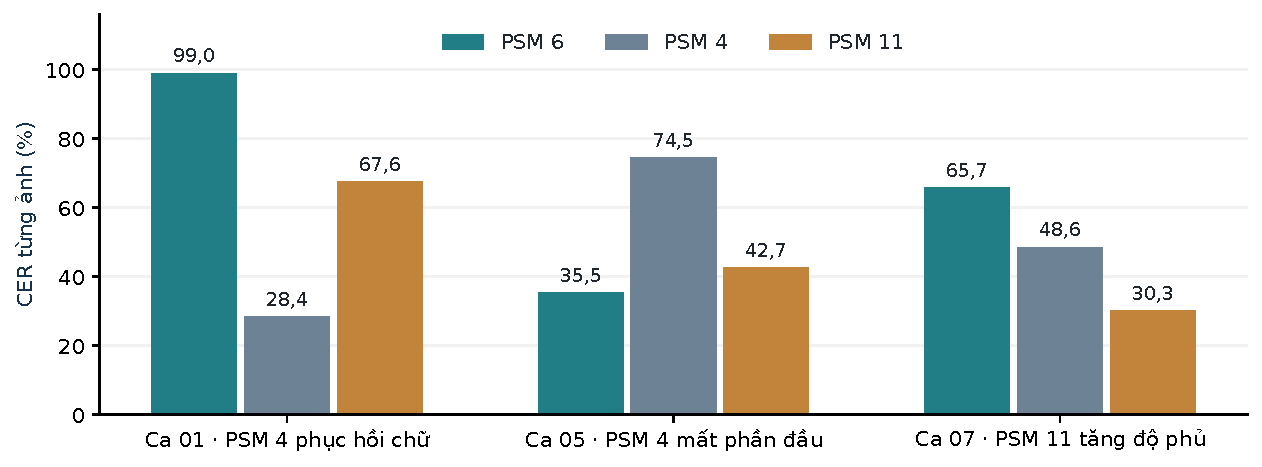
\includegraphics[width=\linewidth]{figures/psm_cases.pdf}
\caption{CER của ba trường hợp được chọn có chủ đích từ phân tích lỗi Goal 2. Sự thay đổi trái chiều giữa các ảnh cho thấy ảnh hưởng của bố cục; mẫu này không đại diện phân bố toàn tập.}\label{fig:psmcases}
\end{figure}

\textbf{Ca 01 và 07: phục hồi nội dung.} Ở ca 01, PSM 6 chỉ phát tám box; PSM 4 phục hồi thêm chữ, giảm CER từ khoảng 99,0\% xuống 28,4\%. Ở ca 07, PSM 11 lấy thêm vùng bảng/header mà PSM 6 biểu diễn kém, nhưng thứ tự từ trong dòng vẫn có lỗi. Điểm giảm không đồng nghĩa toàn bộ dòng đã được nhận dạng đúng.

\textbf{Ca 05: mất phần đầu hóa đơn.} PSM 4 phát 21 box so với 108 box của PSM 6, bỏ phần đầu và làm CER tăng từ khoảng 35,5\% lên 74,5\%. Hiện tượng mất phần đầu đã được xác nhận trong hồ sơ thẩm định. Bất thường về ngày tháng trong nguồn chưa được phân xử nên transcript vẫn được giữ nguyên.

\textbf{Ca 10: ảnh hưởng của thứ tự ghép.} Bốn token trên cùng một dòng có tâm $y$ lần lượt 876,5; 877,0; 878,5; 879,5 pixel. Quy tắc ưu tiên $y$ làm chuỗi được nối khác thứ tự trái sang phải. Truy nguyên cho thấy đóng góp của phép ghép đối với dòng này; kết luận nguyên nhân tổng thể vẫn còn bất định. Thuật toán và điểm benchmark được giữ nguyên.

\textbf{Ca 16 và 17: nguyên nhân chưa được thống nhất.} Ca 16 có chữ nằm ngang và PSM 4 trả danh sách rỗng với trạng thái thành công; chưa tách được nguyên nhân do hướng ảnh hay yếu tố khác. Ca 17 còn bất đồng về giả thuyết GT lệch dòng. Có thể truy nguyên phép gán box vào vùng, nhưng chưa đủ căn cứ kết luận lỗi annotation đã được xác nhận.

\subsection{Mức ổn định của lợi thế PSM 11}
So với PSM 6, CER của PSM 11 tốt hơn trên 110 ảnh, kém hơn trên 108 ảnh và bằng nhau trên 13 ảnh. Phân tích bootstrap ghép cặp 5.000 lần trong hồ sơ cho khoảng 95\% của chênh lệch CER là $[-1{,}696;\,0{,}173]$ điểm phần trăm, của WER là $[-1{,}287;\,0{,}644]$ điểm phần trăm. Cả hai chứa 0. Đây là phân tích thăm dò sau chạy, giả định ảnh độc lập; không loại được sai số annotation hoặc alignment.

Nhóm chọn \textbf{PSM 11 làm ứng viên cho thí nghiệm tiếp theo, giữ PSM 6 làm đối chứng}. Chưa thay mặc định sản phẩm và chưa kết luận PSM 11 tốt nhất cho mọi hóa đơn. PSM 4 cần xem kỹ nguy cơ bỏ dòng hoặc trả rỗng dù có ưu điểm ở một số bố cục.

\clearpage
\section{Goal 3: So sánh ba engine nhận dạng}
\subsection{Phạm vi và cấu hình thí nghiệm}
VietOCR, Tesseract và PaddleOCR chạy tuần tự trên cùng 1.300 crop \texttt{official\_val}, với 23.739 ký tự và 4.815 token tham chiếu. Đây là nhận dạng trên crop có sẵn; PaddleOCR không chạy detector. Theo báo cáo nhóm, mỗi engine thành công 1.300/1.300 crop, không lỗi thực thi và đã vượt kiểm tra tập crop, split và mẫu số.

\begin{table}[H]
\caption{Cấu hình, chất lượng nhận dạng và thời gian thực thi Goal 3 trên 1.300 crop validation. Nguồn: báo cáo thí nghiệm ba engine.}
\small
\begin{tabularx}{\linewidth}{@{}P{30mm}Yrrr@{}}
\toprule
\textbf{Engine} & \textbf{Model} & \textbf{Rỗng} & \textbf{CER} & \textbf{WER}\\\midrule
VietOCR 0.3.13 & \nolinkurl{vgg_transformer} \cite{vietocr} & 0 & \textbf{9,59\%} & \textbf{33,87\%}\\
Tesseract 5.3.4 & Tiếng Việt (\texttt{vie}), PSM 7 & 5 & 19,51\% & 55,49\%\\
PaddleOCR 3.7.0 & \nolinkurl{latin_PP-OCRv5_mobile_rec} \cite{paddleocr} & 5 & 17,44\% & 63,03\%\\
\bottomrule
\end{tabularx}
\vspace{4mm}
\begin{tabularx}{\linewidth}{@{}Yrr@{}}
\toprule
\textbf{Engine} & \textbf{Tổng thời gian (giây)} & \textbf{Trung bình/crop (ms)}\\\midrule
VietOCR & 137,7 & 105,9\\
Tesseract & \textbf{85,7} & \textbf{65,9}\\
PaddleOCR & 207,7 & 159,8\\
\bottomrule
\end{tabularx}
\end{table}

\begin{figure}[H]
\centering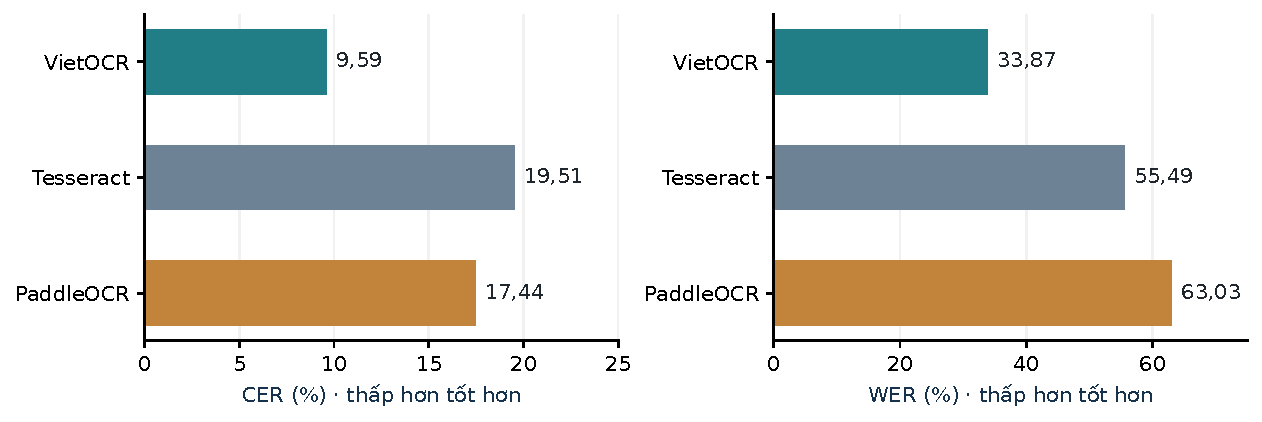
\includegraphics[width=\linewidth]{figures/engine_metrics.pdf}
\caption{Thứ hạng theo CER và WER trên cùng 1.300 crop Goal 3. Hai ô dùng thang đo riêng. Biểu đồ làm rõ việc PaddleOCR và Tesseract đổi thứ hạng giữa hai chỉ số; nguồn: báo cáo nhóm.}
\end{figure}

VietOCR giảm CER khoảng 50,8\% và WER khoảng 39,0\% tương đối so với Tesseract; tương ứng giảm 9,92 và 21,62 điểm phần trăm. PaddleOCR giảm CER khoảng 10,6\% nhưng tăng WER khoảng 13,6\% tương đối. Cần xem cả hai chỉ số: khoảng trắng, dấu câu và lỗi trong token có thể ảnh hưởng kết quả, nhưng chưa có đối chiếu từng crop để xác nhận cơ chế hoặc phân bố lỗi của Goal 3.

\note{\textbf{Giới hạn bằng chứng.} Kết quả Goal 3 được tổng hợp từ báo cáo thí nghiệm của nhóm. Chưa có bộ dự đoán và nhật ký thực thi gốc trong hồ sơ đối chiếu để kiểm chứng độc lập độ phủ mẫu và thời gian. Thời gian còn khác số liệu ở bản ghi trước, nên chỉ được xem là quan sát của lượt chạy được báo cáo.}

\clearpage
\section{Thảo luận và độ tin cậy của kết luận}
\subsection{Phân biệt nhận dạng, ghép vùng và chất lượng nguồn}
Ba goal cùng cho thấy một điểm OCR chỉ có nghĩa khi biết đơn vị chấm và ground truth. Goal 1 loại khâu ghép polygon bằng cách so trực tiếp từng crop. Goal 2 còn phụ thuộc phân đoạn trang, vị trí box, thứ tự nối từ và phần GT có transcript. Goal 3 dùng crop như Goal 1 nhưng có engine, phiên bản và môi trường khác. Không dùng khoảng cách giữa các bảng để tính mức cải thiện chung của dự án.

Phát hiện lỗi parser là kết quả quan trọng của tuần 2: một evaluator có thể tính đúng khoảng cách chỉnh sửa trên một tham chiếu sai. Kiểm thử và checksum giúp phát hiện lỗi thực thi, thay đổi dữ liệu hoặc sai tổng hợp; chúng không tự chứng nhận chữ tham chiếu đúng với ảnh. Vì thế, kiểm tra nguồn và review trực quan cần được duy trì cùng kiểm thử tự động.

\subsection{Đánh đổi độ chính xác và thời gian}
Trong Goal 3, VietOCR đạt độ chính xác tốt nhất theo CER/WER, còn Tesseract có thời gian trung bình/crop thấp nhất của lượt chạy. Chưa đủ cơ sở để khái quát thứ hạng tốc độ vì chưa đối chiếu được cách đo, số luồng, tải máy và số lần lặp. Bản ghi trước ghi trung bình 85,0; 65,2; 99,8 ms/crop cho VietOCR, Tesseract và PaddleOCR, khác 105,9; 65,9; 159,8 ms/crop trong báo cáo thí nghiệm hiện tại. Nguyên nhân chênh lệch cần được làm rõ bằng nhật ký gốc.

Ở Goal 2, tổng thời gian PSM 6/4/11 lần lượt là 96,51/92,51/108,72 giây; trung bình 417,4/400,2/470,3 ms/ảnh. Đây là quan sát đơn lượt, có chi phí khởi động tiến trình, không phải xếp hạng tốc độ có ý nghĩa thống kê. Lựa chọn cấu hình còn phải xét bỏ sót nội dung: PSM 4 nhanh hơn trong lần đo nhưng có 14 ảnh rỗng.

\subsection{Bằng chứng đã có và phần còn hạn chế}
\begin{table}[H]
\caption{Bằng chứng và giới hạn của từng thí nghiệm. Nguồn: hồ sơ Goal 1, Goal 2 và báo cáo thí nghiệm Goal 3.}
\begin{tabularx}{\linewidth}{@{}P{29mm}YY@{}}
\toprule
\textbf{Thành phần} & \textbf{Bằng chứng hiện có} & \textbf{Giới hạn cần giữ}\\\midrule
Goal 1 & Chỉ số từng crop khớp tổng hợp; có kiểm tra dữ liệu và phân tích 24 mẫu. & Nhãn nguồn chưa được phân xử toàn bộ; mẫu lỗi không đại diện.\\
Goal 2 & Kết quả sau sửa nguồn trên 231 ảnh; phân biệt độ phủ chữ và hình học. & GT thiếu chữ ở nhiều vùng; bất định nguyên nhân và thứ tự ghép còn tồn tại.\\
Goal 3 & Các bản tổng hợp thống nhất CER/WER của ba engine. & Chưa đối chiếu dự đoán và nhật ký gốc; thời gian khác bản ghi trước.\\
Khả năng áp dụng & Có cơ sở chọn ứng viên OCR cho bước nghiên cứu tiếp theo. & Chưa có detection F1, field accuracy KIE hay đánh giá end-to-end.\\
\bottomrule
\end{tabularx}
\end{table}

Lượt kiểm chứng Goal 2 ngày 05/11/2026 đạt 167/167 bài kiểm thử và 170 kiểm tra về nguồn dữ liệu, độ phủ và tính lại kết quả. Khoảng cách chỉnh sửa của 12.795 vùng qua ba PSM được đối chiếu bằng một triển khai độc lập. Các kiểm tra này xác nhận tính nhất quán của phép tính; những bất định về nhãn và nguyên nhân lỗi vẫn cần được giải quyết riêng.

\clearpage
\section{Kết luận và hướng tiếp theo}
Tuần 2 đã tạo được baseline crop có phạm vi và mẫu số rõ ràng, sửa một lỗi nguồn ảnh hưởng đến diễn giải OCR toàn trang, đồng thời có kết quả so sánh ba engine trên cùng bộ crop. Giá trị chính là kết nối số đo với điều kiện thực nghiệm và bằng chứng lỗi, từ đó tránh lựa chọn cấu hình chỉ theo một chỉ số tổng hợp.

VietOCR là ứng viên ưu tiên cho bước nhận dạng tiếp theo dựa trên CER/WER Goal 3. Với Tesseract toàn trang, PSM 11 là ứng viên cần thử thêm và PSM 6 tiếp tục làm đối chứng. Đây là định hướng nghiên cứu có điều kiện; chưa xác nhận kiến trúc cuối cùng hoặc chất lượng trích xuất trường của sản phẩm.

\begin{table}[H]
\caption{Các bước tiếp theo và tiêu chí kiểm tra dự kiến; chưa phải kết quả đã hoàn thành.}
\begin{tabularx}{\linewidth}{@{}P{8mm}YY@{}}
\toprule
\textbf{Ưu tiên} & \textbf{Công việc} & \textbf{Tiêu chí đối chiếu}\\\midrule
1 & Hoàn thiện hồ sơ thực nghiệm Goal 3 và quy ước đo thời gian. & Khớp ID, mẫu số, dự đoán và model; cách đo, số luồng rõ ràng, đo lặp cùng điều kiện.\\
2 & Phân xử các ca transcript/geometry còn bất định. & Có quyết định theo từng ca, phiên bản nhãn và lịch sử sửa; giữ split đã khóa.\\
3 & Thử cải tiến thứ tự ghép dòng và xử lý hướng ảnh trên dev. & Tách từng thay đổi, so với baseline cố định; đo cả điểm chữ và coverage.\\
4 & Ghép detector với VietOCR và đánh giá end-to-end. & Chấm vùng chữ và nội dung trên dữ liệu phù hợp; sau đó mới đo từng trường KIE.\\
\bottomrule
\end{tabularx}
\end{table}

Quá trình chọn mô hình và tham số tiếp theo cần dùng dữ liệu phát triển tách từ train. Khi chuyển sang KIE, nhãn trường phải được kiểm tra riêng; transcript crop không tự trở thành nhãn tên nơi bán, thời gian hoặc tổng tiền. Các ví dụ review hiện có là đầu vào cho phân xử và thiết kế thí nghiệm, không thay thế tập đánh giá đại diện.

\clearpage
\begin{thebibliography}{99}
\setlength{\itemsep}{10pt}
\bibitem{mcocr} Ban tổ chức MC-OCR. \textit{Mobile-Captured Image Document Recognition for Vietnamese Receipts.} RIVF 2021. Trang chính thức về dữ liệu và tác vụ.\\
\href{https://www.rivf2021-mc-ocr.vietnlp.com/}{\textsf{rivf2021-mc-ocr.vietnlp.com}}. Truy cập: 06/11/2026.
\bibitem{tesseract} Nhóm phát triển Tesseract OCR. \textit{Improving the quality of the output}, mục ``Page segmentation method''. Tài liệu chính thức về các chế độ PSM.\\
\href{https://tesseract-ocr.github.io/tessdoc/ImproveQuality.html\#page-segmentation-method}{\textsf{Tesseract Documentation: Page segmentation method}}. Truy cập: 06/11/2026.
\bibitem{vietocr} pbcquoc và cộng tác viên. \textit{VietOCR: Transformer OCR}, mục ``Model Zoo''. Kho mã nguồn gốc và cấu hình mô hình.\\
\href{https://github.com/pbcquoc/vietocr\#model-zoo}{\textsf{github.com/pbcquoc/vietocr}}. Truy cập: 06/11/2026.
\bibitem{paddleocr} Nhóm phát triển PaddleOCR, PaddlePaddle. \textit{Text Recognition Module}. Tài liệu chính thức về mô hình và mô-đun nhận dạng chữ.\\
\href{https://www.paddleocr.ai/main/en/version3.x/module_usage/text_recognition.html}{\textsf{PaddleOCR Documentation: Text Recognition Module}}. Truy cập: 06/11/2026.
\bibitem{jiwer} Jitsi và cộng tác viên. \textit{JiWER: Process API reference}. Tài liệu định nghĩa và cách tổng hợp CER/WER từ khoảng cách chỉnh sửa.\\
\href{https://jitsi.github.io/jiwer/reference/process/}{\textsf{jitsi.github.io/jiwer/reference/process}}. Truy cập: 06/11/2026.
\end{thebibliography}

\end{document}

